\documentclass[10pt,a4paper]{report}

\usepackage[utf8]{inputenc}
\usepackage{amsmath}
\usepackage{amsfonts}
\usepackage{amssymb}
\usepackage{graphicx}
\usepackage{color}
\usepackage{enumitem}

\usepackage[top=1cm, bottom=2cm, left=2cm, right=2cm]{geometry}
\usepackage{hyperref}
\usepackage{fancyhdr}
\pagestyle{fancy}

\fancyhead{}
\fancyfoot{} 
\lhead{ \hspace{0.1cm} M1 WI 2014-2015  \hspace{0.4cm} \vline}
\chead{Interoperabilité}
\rhead{K.B - B.B - K.L - N.R}
\rfoot{\thepage}

\author{Kevin BASCOL, Bachir BOUACHERIA, Kevin LAOUSSING, Nicolas REYNAUD}
\title{ Interopérabilité: Find Your Way}

\makeatletter
\renewcommand{\thesection}{\@arabic\c@section}
\makeatother

\begin{document}

\makeatletter
	\begin{titlepage}
	
	\centering
		{
		\vspace*{5cm}
		\hrule height 2pt
		\vspace{0.7cm}
		\Huge \textbf{\@title}}\\
		\vspace{0.7cm}
		\hrule height 2pt
		
		\vfill
		\vspace{1cm}
		\@author\\
		\end{titlepage}
\makeatother
\setcounter{secnumdepth}{4}
\setcounter{tocdepth}{3}
\renewcommand{\contentsname}{Sommaire}
\begingroup\makeatletter
\def\@makeschapterhead#1{%
  {\parindent \z@ \raggedright
    \normalfont
    \interlinepenalty\@M
    \Huge \bfseries  #1\par\nobreak
    \vskip 20pt% <---- à réduire pour avoir plus de place
  }}\makeatother
\tableofcontents
\endgroup
\thispagestyle{empty}
\setcounter{page}{0}
\newpage

\newgeometry{top=2cm, bottom=2cm, left=2cm, right=2cm}

%%%%%%%%%%%%%%%%%%%%%%%%%%%%%%%%%%%%%%%%%%%%%%%%%%%%%%%
%%%					INTRODUCTION					%%%
%%%%%%%%%%%%%%%%%%%%%%%%%%%%%%%%%%%%%%%%%%%%%%%%%%%%%%%
\section{Introduction}

\subsection{Description du projet}
\begin{flushleft}
\textbf{Find your way} est un logiciel de type "smart-cities" permettant de localiser toutes les activités à proximité de la position de l'utilisateur, dans un rayon donné pour celui-ci.\\
Parmi les activités localisées par le logiciel, on y trouve les cinéma, les librairie, les bars, et les restaurants. Pour chacune de ses activités, le logiciel est capable de réunir des informations utiles tel que les prix des menus d'un restaurant désigné par l'utilisateur, les horaires des séances d'un film pour un cinéma donné, etc.
\textbf{Find your way} utilise plusieurs sources de données et de format différents, qui justifie sa composante d'interopérabilité. On y trouve des données de géolocalisation, des données extraites des pages web de site internet, en plus d'utiliser des données stockées dans une base de donnée que les utilisateurs peuvent compléter.
Ce rapport présentera dans un premier temps la fonctionnalité de géolocalisation de l'utilisateur et des activités à proximité de celui-ci. Puis dans un deuxième temps, la recherche d'information pour des divers activités localisés. Dans un troisième temps, une description du système d'introduction d'information par l'utilisateur dans la base de donnée du logiciel.

\end{flushleft}

\subsection{Outils et supports}

\begin{flushleft}
\textbf{Find your way} est une application web réalisée avec divers outils et supports décrient dans cette liste :

\begin{itemize}

\item API Google Map V3 à retrouver a se lien :
\begin{verbatim}
	https://developers.google.com/maps/documentation/javascript/
\end{verbatim} 

\item Framework x?  à complete Bachir

\item Langage PHP, javascript, HTML, CSS. 

\end{itemize}
\end{flushleft}

%%%%%%%%%%%%%%%%%%%%%%%%%%%%%%%%%%%%%%%%%%%%%%%%%%%%%%%
%%%					GEOLOCALISATION					%%%
%%%%%%%%%%%%%%%%%%%%%%%%%%%%%%%%%%%%%%%%%%%%%%%%%%%%%%%

\section{La géolocalisation}

\subsection{Description de la fonctionnalité}
\begin{flushleft}
La géolocalisation nous permet de savoir avec plus ou moins d'exactitude la position d'une personne. Ceci ayant pour but de pouvoir identifier a l'aide des API Google map les lieux a proximité d'une personne. \\

Il s'agit de la base de notre concepte, pouvoir localiser une personne.
\end{flushleft}

\subsection{Description technique}
\begin{flushleft}
La géolocalisation se fait a l'aide de l'HTML5 et ses nouvelles fonctionnalité. Nous passons ensuite les informations a gooogle map pour avoir la liste des lieux a proximité de la personne dans un rayon donné. \\
Nous obtenons alors une liste de lieu dans le format JSon que nous devons interpréter et retirer les bonnes informations.\\
Ses lieux sont ensuite affiché sur la carte à l'aide marqueur. Grâce a du Javascript. \\

Pour le calcule de distance, nous avons du implémenter ceci : 
\begin{verbatim}
	http://fr.wikipedia.org/wiki/Distance_entre_deux_points_sur_le_plan_cart%C3%A9sien$ 
\end{verbatim}
\end{flushleft}


%%%%%%%%%%%%%%%%%%%%%%%%%%%%%%%%%%%%%%%%%%%%%%%%%%%%%%%
%%%					RECHERCHE INTERNET				%%%
%%%%%%%%%%%%%%%%%%%%%%%%%%%%%%%%%%%%%%%%%%%%%%%%%%%%%%%

\section{Recherche d'information sur internet}

\subsection{Description de la fonctionnalité}
\begin{flushleft}
Lorsque les activités à proximité de l'utilisateur sont localisées, celui-ci à la possibilité de choisir les activités dont il aimerait obtenir plus d'information.
Par exemple, si l'utilisateur décide d'obtenir des informations sur les horaires des séances des films d'un cinéma, il lui suffit de cliquer sur le cinéma qui l’intéresse et le logiciel se chargera de lui apporter les informations demandées.
\textbf{Find your way} va alors visiter le site web correspondant à l'activité ( dans l'exemple d'une activité de type cinéma, il va consulter le site \url{http://www.allocine.fr/} ) et extraire les informations des pages web du site.\linebreak

Les sites web consultés par \textbf{Find your way} en fonction de l'activité :

\begin{itemize}
\item Cinéma : \url{http://www.allocine.fr/}.

\item Livre : \url{http://livre.fnac.com/}.

\item Restaurant et bar : leur propre site web ( si ceux-ci sont référencés sur internet).

\end{itemize}
\end{flushleft}

\subsection{Description technique}
\begin{flushleft}
Pour extraire l'information des pages web, \textbf{Find your way} un programme PHP qui va récuperer la page web en tant que chaine de caractère. Puis il utilise des expressions régulières pour filtrer et trouver les bonnes balises HTML contenant les informations à extraire.\newline

Exemple :
 Sur ce \href{http://www.allocine.fr/seance/salle_gen_csalle=P0231.html}{lien}, \textbf{Find your way} cherche à récuperer toute les titres des films à l'affiche. \\
 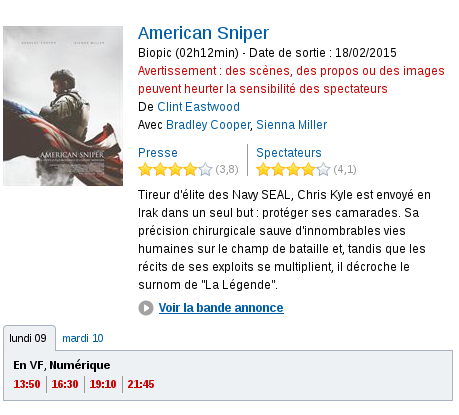
\includegraphics[scale=0.45]{./images/allocine_img1.png}
 
 Pour se faire il analyse le code source de la page html et reconnaît la chaîne de caractères (cadre bleu)  et récupère le titre (cadre rouge)\\
  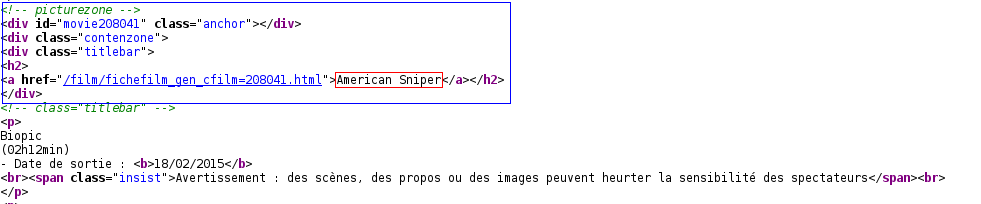
\includegraphics[scale=0.45]{./images/allocine_img2.png}
 avec cette expression régulière : \\
 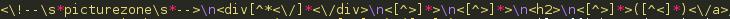
\includegraphics[scale=0.45]{./images/allocine_img3.png}
\end{flushleft}

%%%%%%%%%%%%%%%%%%%%%%%%%%%%%%%%%%%%%%%%%%%%%%%%%%%%%%%
%%%					BASE DE DONNEE					%%%
%%%%%%%%%%%%%%%%%%%%%%%%%%%%%%%%%%%%%%%%%%%%%%%%%%%%%%%

\section{Base de donnée}

\subsection{Description de la fonctionnalité}
\begin{flushleft}
Pour ajouter des lieux et avoir le suivit des votes, nous devons stocker tout ceci dans le base de donnée afin de pouvoir retourner les informations en temps voulu. \\

Les votes sont stocké par Ip et par article. \\
\end{flushleft}

\subsection{Description technique}
\begin{flushleft}
Pour effectuer les votes, nous avons du à l'aide du php, récupérer l'ip de la personne qui vote. Ainsi nous pouvons limiter le nombre de vote par ip et pas lieu. \\

Pour ajouter un lieu, nous récupérons la positon de la personne, puis encore une fois a l'aide des API google map qui inverse la géolocalisation ( de coordonnée donne une adresse ). Nous pouvons alors ajouter le lieu en base de donnée avec le nom fournit par l'utilisateur. \\

Lors de l'affichage nous devons encore une fois implémenter 
\begin{verbatim}
	http://fr.wikipedia.org/wiki/Distance_entre_deux_points_sur_le_plan_cart%C3%A9sien
\end{verbatim} 
pour cause, nous devons savoir a combien de metre nous somme du nouveau lieu.
Si le lieu est dans  notre périmètre alors nous l'affichons.\\
\end{flushleft}


%%%%%%%%%%%%%%%%%%%%%%%%%%%%%%%%%%%%%%%%%%%%%%%%%%%%%%%
%%%						CONCLUSION					%%%
%%%%%%%%%%%%%%%%%%%%%%%%%%%%%%%%%%%%%%%%%%%%%%%%%%%%%%%

\section{Conclusion}
\begin{flushleft}
•
\end{flushleft}
\end{document}
